\section{Description}
This method uses stochastic event sets and associated ground motion fields to compute loss curves for each asset contained in an exposure file, as illustrated in the following scheme:  

\begin{figure}[ht]
\centering
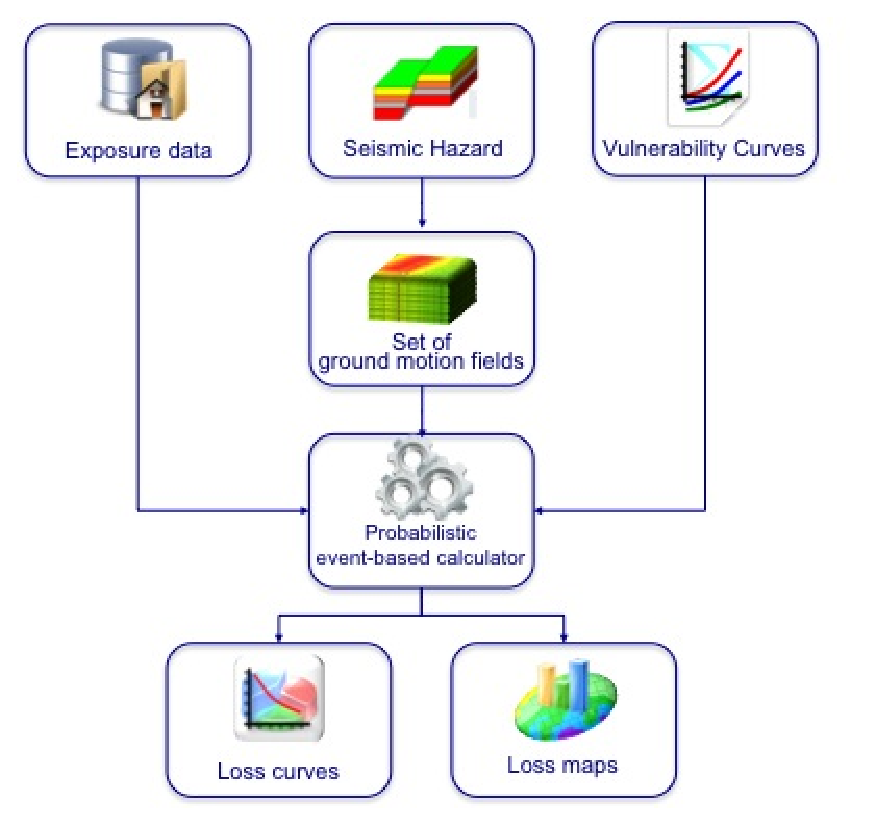
\includegraphics[width=9cm,height=10cm]{./Figures/Part_Risk/Scheme_Prob_calc.eps}
\caption{Architecture of the probabilistic event-based calculator.}
\label{fig:Scheme_Prob_calc}
\end{figure}

For each ground motion field, the intensity measure level at a given site is used to calculate the mean loss ratio using the vulnerability functions for each asset defined in the exposure file. The occurrence distribution of mean loss for a given asset is calculated using all of the ground motion fields, leading to a histogram of loss ratios which is then converted into a cumulative histogram, by calculating the number of cumulative occurrences for each interval of loss ratio. The rate of exceedance of each loss ratio is calculated by dividing the number of cumulative occurrences by the number of stochastic event sets multiplied by the length of each event set. By assuming a Poissionian distribution of the occurrence model, the probability of exceedance of each loss ratio is calculated. 
 
\par \ 

\par
 
If an aggregated loss curve for a portfolio of assets is required, a secondary module is required in order to aggregate the losses from all the assets in the exposure file, per event, before calculating the occurrence distribution of mean loss. If the assets are close enough, it is necessary to generate the ground motion fields taking into account the spatial correlation of ground motion residuals. 

\section{Calculations workflow}

\begin{enumerate}
\item The first step is to compute the loss ratios per asset. In order to do so, the  engine uses the set of ground motion fields to extract the intensity measure levels for the location of each asset. Given this set of values and the respective vulnerability function, the distribution of loss ratios is computed. 

\item In this method an histogram of the loss ratios per asset is required. Before the histogram can be built, it is necessary to define the number and width of the bins. The former might vary significantly since it might depend of several factors (e.g. number of ground motion fields, range of ground motion covered by the vulnerability model) while the later is related with the minimum and maximum values of loss ratio previously computed and with the number of bins. 

\item The histograms for each asset need to be converted into a cumulative histogram. The number of occurrences for each bin can be derived using the following formula:

\begin{equation}
NCO_m = \sum_{n=m} NO_n
\end{equation}

where $NCO_m$ stands for the number of cumulative occurrences of the $m^{th}$ bin of the cumulative histogram and $NO_n$ stands for the number o occurrences of the $n^{th}$ bin of the histogram of the loss ratios.

\item Thereafter, the rate of exceedance of a set of loss ratios needs to be computed for each asset. This set of loss ratios is composed by the middle values of each bin of the cumulative histogram. The following formula is employed to compute this rate:

\begin{equation}
\lambda(LR_n) = \frac{NCO_n}{TSES}
\end{equation}

Where $\lambda$ stands for the rate of exceedance of the respective loss ratio and $TSES$ stands for the time representative of the stochastic event set which means, the number of stochastic event sets multiplied by the time span of each one.

\item Assuming a poissonion distribution of the occurrence model, the probability of exceedance of the set of loss ratios can be derived using the following formula:

\begin{equation}
PE(LR_n) = 1-\exp{-\lambda_n\times t}
\end{equation}

Where $t$ stands for the time span used to produce the stochastic event set.

\end{enumerate}









